\begin{figure}[ht] % Inline image example
\begin{center}
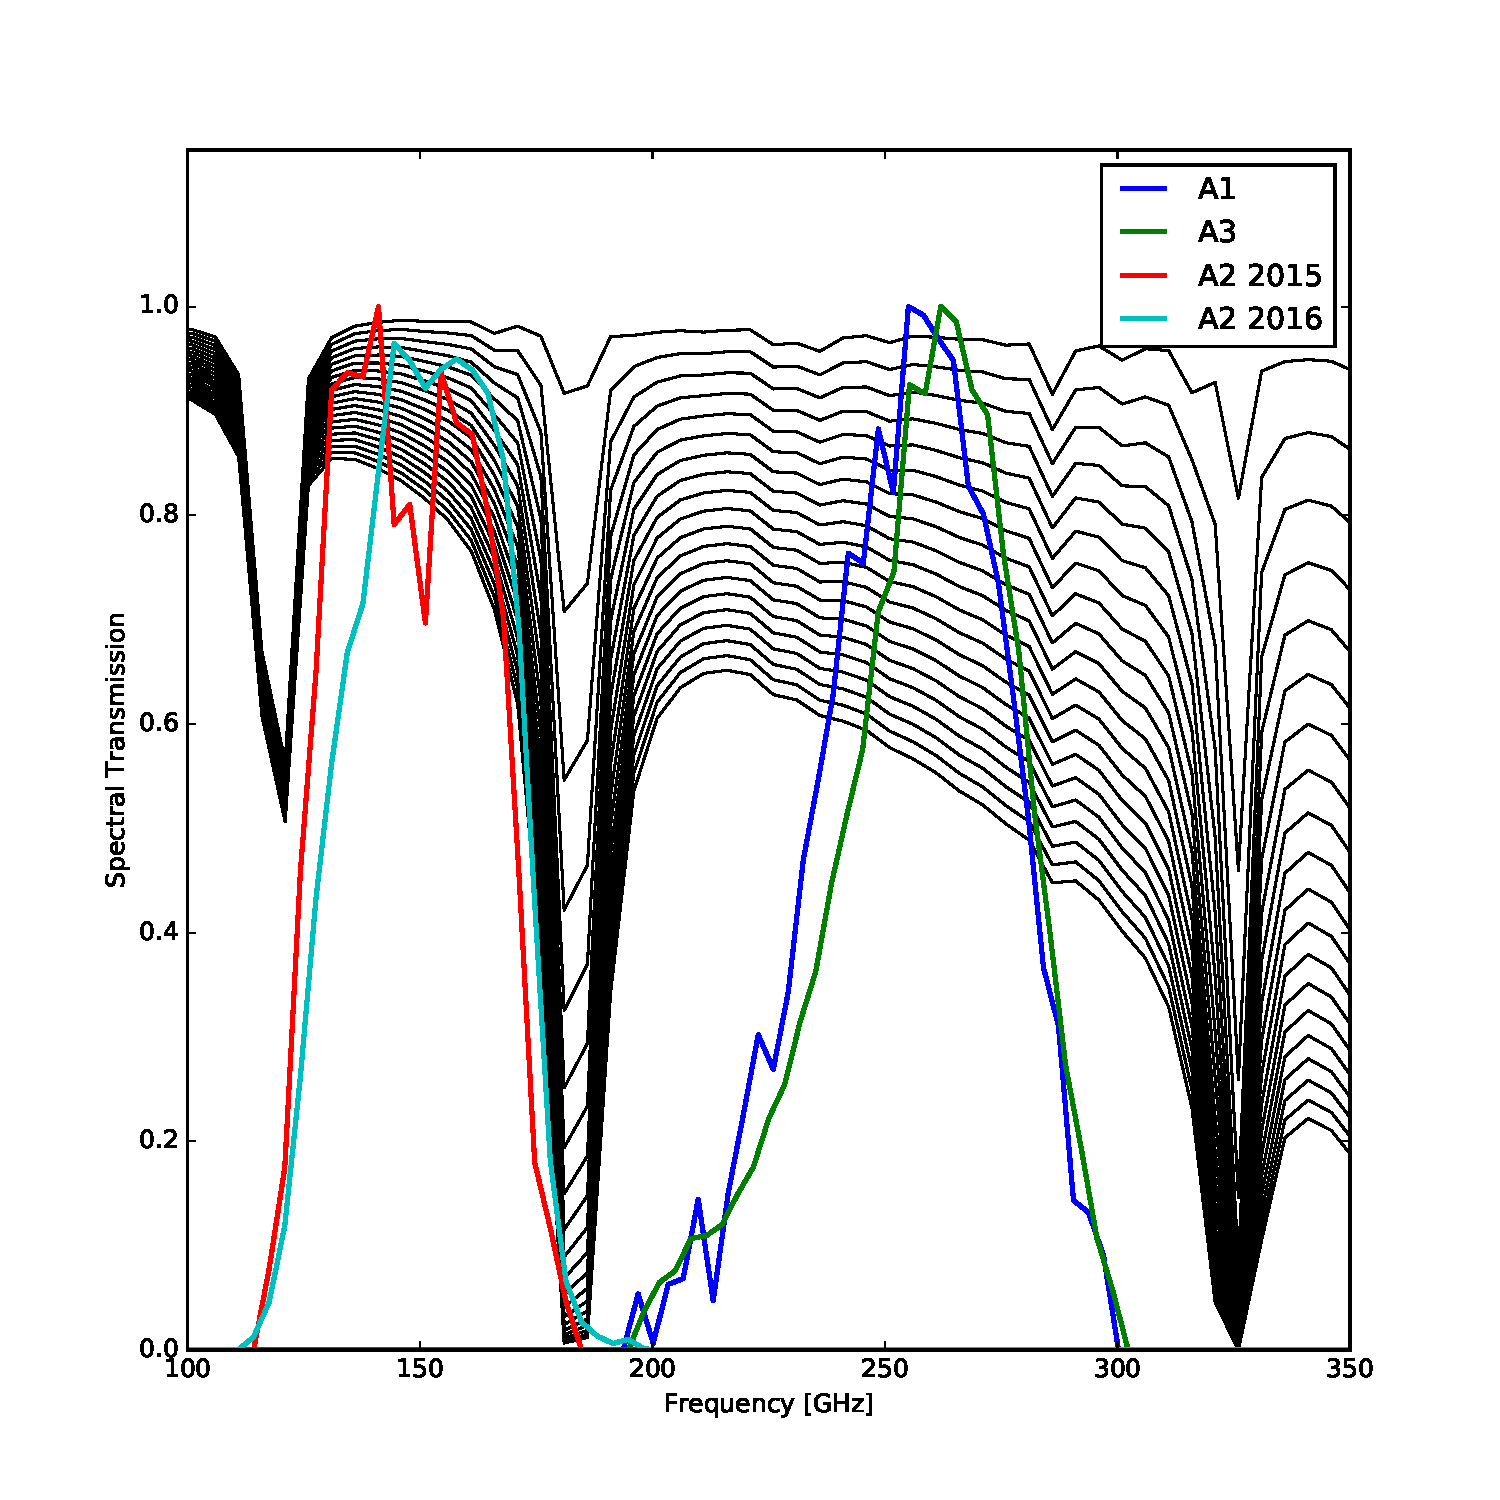
\includegraphics[width=\textwidth]{Figures/SpectralBands/atm_transmission.pdf}
\end{center}
\caption{Spectral transmission of the the three NIKA2 arrays as a function of frequency in GHz. For illustration we also plot the ATM atmospheric model for different values of pwv. \label{spectralband}}
\end{figure}




The NIKA2 spectral bands were measured in the laboratory using a Martin Pupplet interferometer.
Both arrays and filter bands were considered in the measurements. Theser were obtained from the difference of two black-bodies, hence they include a a $\nu^2$ RJ term. During the commissioning in Run 5 array 2 was replaced. The new array has a different spectral transmission. Figure shows the spectral transmissions for the three arrays. Notice that array A2 was replaced by a new on in N2R5 and that the spectral transmissions are not the same (red and cyan lines in the figure).


\begin{table}[h]
\caption{Spectral transmission characteristics for the NIKA2 arrays.%
\label{nika2runs}}
\begin{tabular}{|c|c|c|c|c|}
\hline 
  &     A1  &  A3 &  A2 2015 & A2 2016 \\ 
\hline 
Central Frequency [GHz] &   255.5  & 257.8   &   147.7  & 151.6 \\  
Bandwidth [GHz]         &   47.8   & 45,7    &   41.8   & 42.1 \\
\hline 
\end{tabular} 
\end{table} 


What actually matters more than the ``central frequency'' that depends on many
assumptions and definitions are the bandpasses. We should make available in a
.fits file, clearly, our bandpasses to avoid future misunderstanding and propagation of
false numbers. Official values should be 150 and 260~GHz. We should also clearly
state that these measured bandpasses were done with the difference of two
black-bodies, hence they include a $\nu^2$ RJ term.\\

With these bandpasses and an official ATM spectrum, we expect an opacity ratio of
XX between 1 and 2mm and see~\ref{se:opacities} for more details.


